\begin{spacing}{1.2}
	\chapter{PENGUJIAN, ANALISIS, DAN PERBANDINGAN}
	\label{sec:chap4_analisis}
\end{spacing}

\vspace{4ex}

Bab ini akan menunjukkan hasil pengujian dari sistem yang telah dibangun, kemudian dilakukan analisis terhadap hasil tersebut yang akan dijadikan bahan perbandingan dengan penelitian terdahulu. Mulai dari hasil pelatihan model hingga pengujian deteksi pada kejadian nyata sehingga diperoleh perbedaan serta hal-hal yang menjadi penyebab muncul perbedaan sistem antara penelitian ini dengan penelitian terdahulu.

\section{Alur Pengujian}
Alur pengujian beserta analisis perbandingan akan dijelaskan secara runtut sebagai berikut:

\begin{enumerate}
    \item Pengujian Model terhadap Deteksi Kendaraan
    \item Pengujian Sistem terhadap Kecepatan Rata-rata 20Km/H pada Siang Hari
    \item Pengujian Sistem terhadap Kecepatan Rata-rata 40Km/H pada Siang Hari
    \item Pengujian Sistem terhadap Kecepatan Rata-rata 20Km/H pada Malam Hari
    \item Pengujian Sistem terhadap Kecepatan Rata-rata 40Km/H pada Malam Hari
    \item Analisis Kualitas terhadap sistem
\end{enumerate}

\section{Pengujian Model terhadap Deteksi Kendaraan}
Penelitian ini terdapat dua model yang telah dikembangkan, yaitu model deteksi kendaraan pada kondisi siang hari, dan kondisi malam hari.

\subsection{Model Deteksi Siang Hari}
Pelatihan model dengan kondisi siang hari yang menggunakan YOLOv8 telah dilakukan sebanyak 250 epoch, dengan setiap epoch memiliki \emph{value} yang berbeda-beda terhadap hasil akurasinya. Tabel akurasi hasil pelatihan model dapat dilihat pada Tabel \ref{table:akurasi model siang}.

\begin{table}[H]
	\caption{Akurasi Hasil Pelatihan Model pada Siang Hari}
    \label{table:akurasi model siang}
	\centering
	\begin{tabular}{|c|c|c|c|}
		\hline
		Epochs & Precision & Recall & mAP50 \\ \hline
		50 & 0.67893 & 0.68114 & 0.6863 \\ \hline
		100 & 0.76356 & 0.77383 & 0.72166  \\ \hline
		160 (\emph{best}) & 0.80555 & 0.79315 & 0.82471  \\ \hline
		200 & 0.79412 & 0.76758 & 0.77683 \\ \hline
		250 & 0.79412 & 0.76758 & 0.77683 \\ \hline
	\end{tabular}
\end{table}

Setelah dilakukan pelatihan didapatkan beberapa grafik yang menunjukkan tingkat akurasi dari model hasil pelatihan yang telah dibuat. Grafik hasil pelatihan model siang dapat dilihat pada Gambar \ref{fig:grafik model siang}.
\begin{figure} [H] \centering
  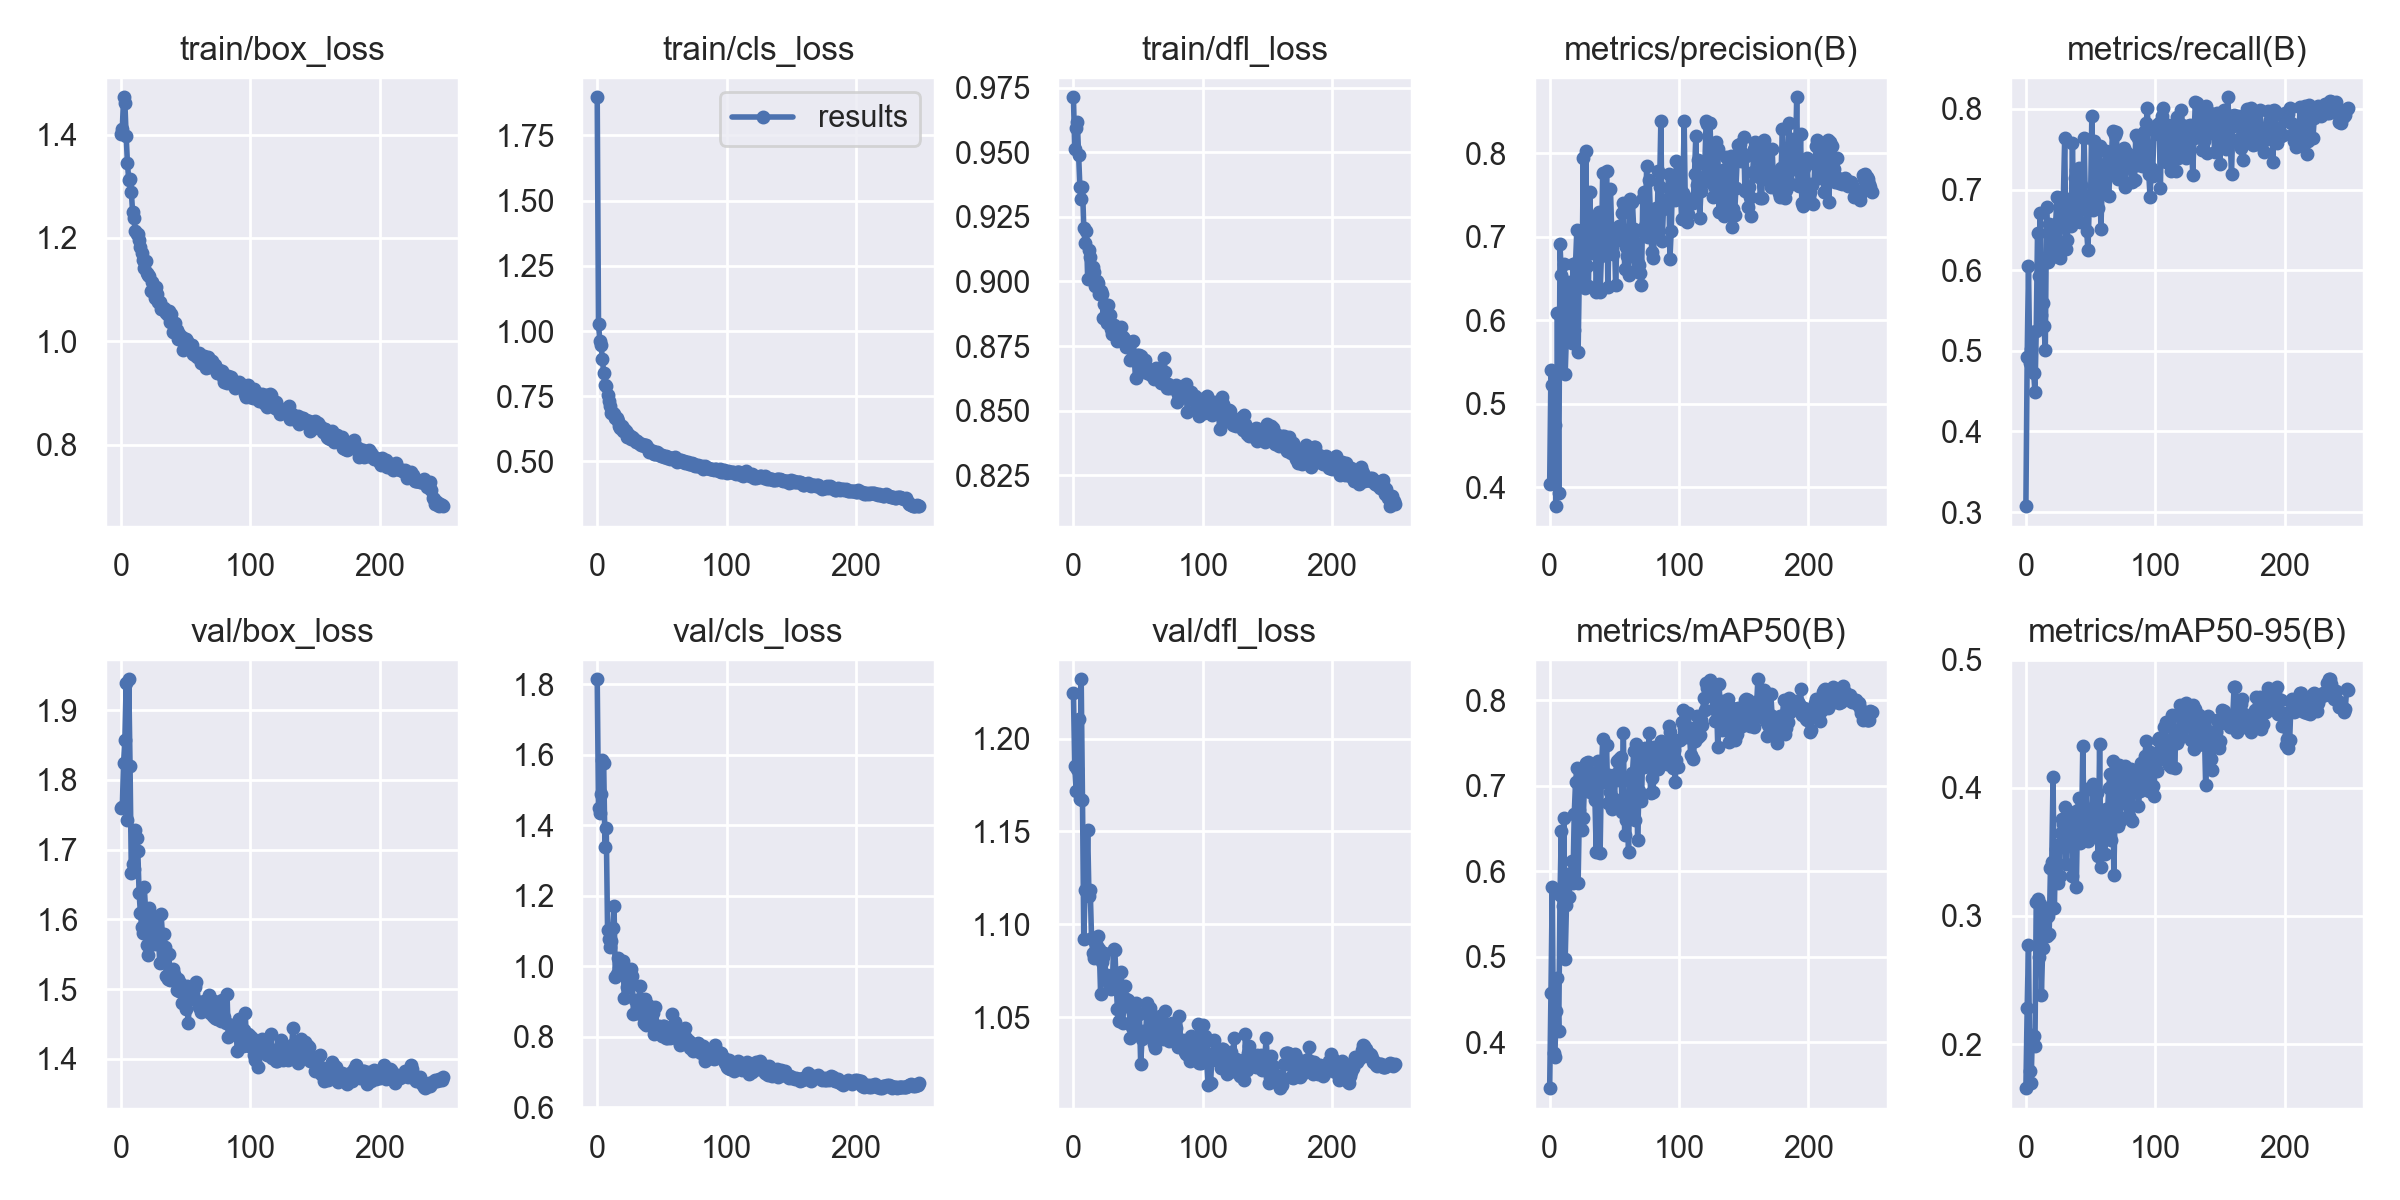
\includegraphics[scale=0.5]{bab4/results_siang.png}
  \caption{Grafik Hasil Pelatihan Model pada Siang Hari}
  \label{fig:grafik model siang}
\end{figure}
Gambar \ref{fig:grafik model siang} menunjukkan kurva hasil pelatihan model YOLOv8 selama 250 epoch. Grafik \emph{train/box\_loss} dan \emph{val/box\_loss} menggambarkan penurunan \emph{bounding box loss} secara konsisten baik pada data pelatihan maupun validasi, yang mengindikasikan bahwa model semakin akurat dalam menentukan lokasi objek. Penurunan serupa juga terlihat pada \emph{train/cls\_loss} dan \emph{val/cls\_loss}, yang merefleksikan peningkatan kemampuan model dalam mengklasifikasikan objek dengan benar. Selain itu, distribusi nilai prediksi model terhadap ground truth yang diukur melalui \emph{train/dfl\_loss} dan \emph{val/dfl\_loss} juga menunjukkan perbaikan yang stabil, menandakan bahwa prediksi model semakin mendekati nilai yang sebenarnya.

Grafik \emph{precision} dan \emph{recall} menunjukkan peningkatan yang signifikan seiring bertambahnya jumlah epoch, hingga mendekati nilai maksimum, yang berarti model semakin andal dalam mendeteksi objek secara akurat dan konsisten. Sementara itu, metrik mAP50 dan mAP50-95 juga memperlihatkan tren kenaikan yang stabil meskipun terdapat fluktuasi kecil, hal ini mencerminkan performa model yang semakin baik dalam berbagai tingkat ambang IoU. Secara keseluruhan, grafik-grafik tersebut memperlihatkan proses pelatihan yang berhasil, dengan peningkatan akurasi deteksi dan penurunan nilai loss yang menunjukkan bahwa model belajar secara efektif dari waktu ke waktu.

Dari hasil pelatihan model siang didapatkan juga confusion matrix yang dapat dilihat pada Gambar \ref{fig:confusion matrix siang}. \emph{Confusion matrix} yang dihasilkan merupakan fitur yang disediakan Ultralytics, sehingga dapat diketahui akurasi setiap \emph{class} yang dijadikan objek deteksi.

\begin{figure} [H] \centering
  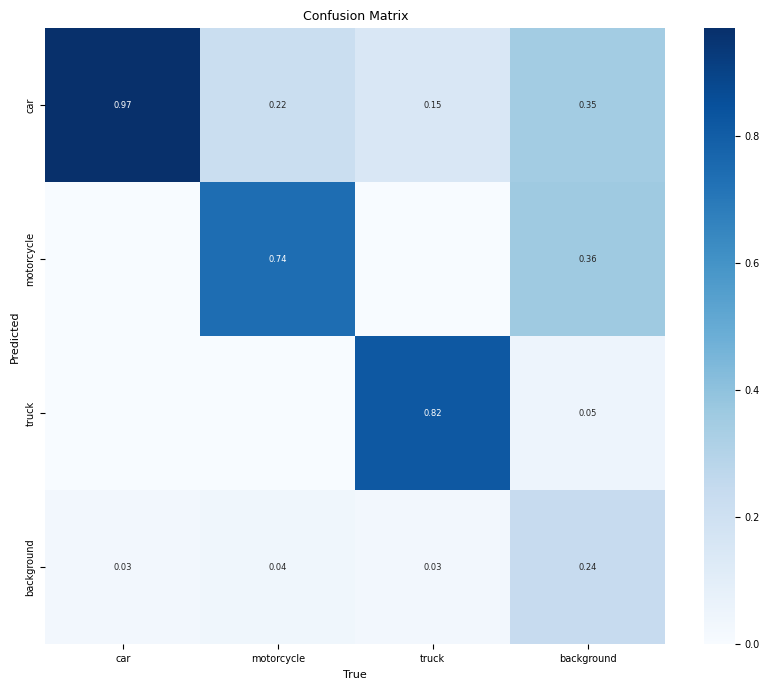
\includegraphics[scale=0.8]{bab4/confusion_siang.png}
  \caption{Confusion Matrix Model Siang Hari}
  \label{fig:confusion matrix siang}
\end{figure}
Pada Gambar \ref{fig:confusion matrix siang} menunjukkan confusion matrix dari hasil pelatihan model YOLOv8 pada kondisi siang hari. Setiap baris pada matriks ini merepresentasikan kelas yang diprediksi oleh model, sementara setiap kolom menunjukkan kelas sebenarnya dari objek yang terdeteksi. Matriks ini memberikan gambaran performa model dalam mengklasifikasikan empat kategori objek, yaitu \emph{car}, \emph{motorcycle}, \emph{truck}, dan \emph{background}.

\begin{enumerate}[nosep]
	\item Kelas \emph{car}:
	Model mengenali objek \emph{car} dengan cukup baik (97\% benar), meski masih ada yang salah dikira \emph{truck} (9\%) dan \emph{background} (22\%).

	\item Kelas \emph{motorcycle}:
	Sebanyak 74\% objek \emph{motorcycle} berhasil dikenali, tapi cukup banyak yang salah diprediksi sebagai \emph{background} (25\%).

	\item Kelas \emph{truck}:
	Akurasi pada kelas \emph{truck} juga tinggi (82\%), namun masih ada kesalahan kecil ke \emph{background} dan \emph{car} (9\%).

	\item \emph{background}:
	Model tampak kesulitan membedakan latar, dengan 33\% \emph{motorcycle} dan 22\% pada \emph{truck} diprediksi \emph{background}.
\end{enumerate}

Secara keseluruhan, model menunjukkan performa terbaik pada kelas \emph{car}, namun masih memerlukan perbaikan dalam mengidentifikasi objek \emph{motorcycle} dan \emph{background}, terutama untuk mengurangi tingkat kesalahan klasifikasi yang tinggi terhadap latar belakang.

Terdapat tahap validasi deteksi objek dari hasil pelatihan model siang yang telah dilakukan. Pada Gambar \ref{fig:validasi deteksi siang} dapat dilihat hasil deteksi dari model pelatihan beserta \emph{confidence threshold} yang diperoleh setiap objek deteksi.

\begin{figure} [H] \centering
  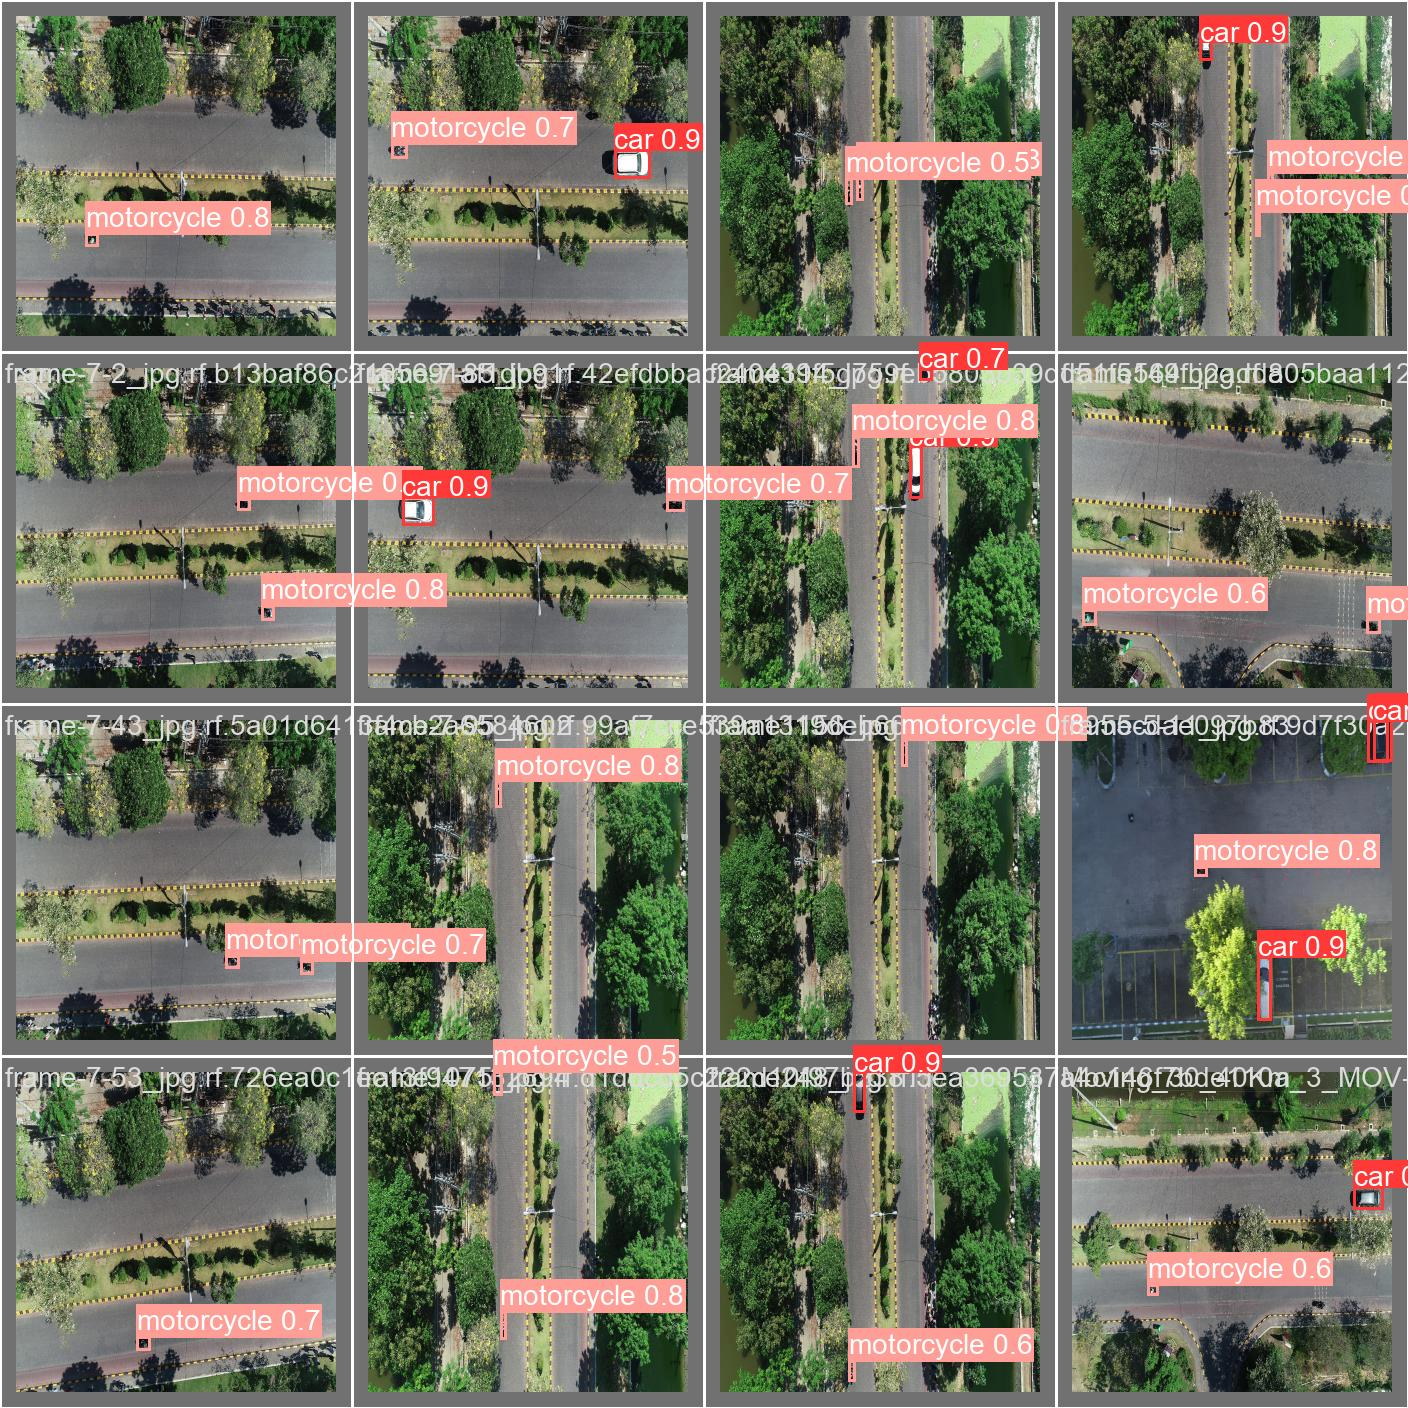
\includegraphics[scale=0.25]{bab4/val_batch_siang.jpg}
  \caption{Validasi Deteksi Siang Hari}
  \label{fig:validasi deteksi siang}
\end{figure}

Dari hasil validasi didapatkan \emph{confidence threshold} untuk setiap objek terdeteksi diatas 0.5 dan ada dua objek motor terdeteksi yang mendapatkan 0.5.

\subsection{Model Deteksi Malam Hari}
Pelatihan model pada kondisi malam hari menggunakan YOLOv8 telah dilakukan selama 250 epoch, di mana setiap epoch menghasilkan \emph{value} akurasi yang bervariasi. Hasil akurasi dari proses pelatihan model tersebut disajikan pada Tabel \ref{table:akurasi model malam}.
\begin{table}[H]
	\caption{Akurasi Hasil Pelatihan Model pada Malam Hari}
    \label{table:akurasi model malam}
	\centering
	\begin{tabular}{|c|c|c|c|}
		\hline
		Epochs & Precision & Recall & mAP50 \\ \hline
		50 & 0.81247 & 0.8977 & 0.81938 \\ \hline
        72 (\emph{best}) & 0.94688 & 0.88395 & 0.92997 \\ \hline
		100 & 0.95264 & 0.88435 & 0.90664 \\ \hline
		200 & 0.9409 & 0.89202 & 0.906 \\ \hline
		250 & 0.92616 & 0.88637 & 0.88913 \\ \hline
	\end{tabular}
\end{table}

Dari hasil pelatihan model juga didapatkan grafik untuk setiap aspek yang diuji sehingga dapat dilihat apakah hasil model sudah sesuai yang diharapkan atau tidak. Grafik hasil pelatihan tersebut dapat dilihat pada Gambar \ref{fig:grafik model malam}. Hasil tersebut dapat digunakan sebagai acuan seberapa besar akurasi model hasil pelatihan yang telah dilakukan.

\begin{figure} [H] \centering
  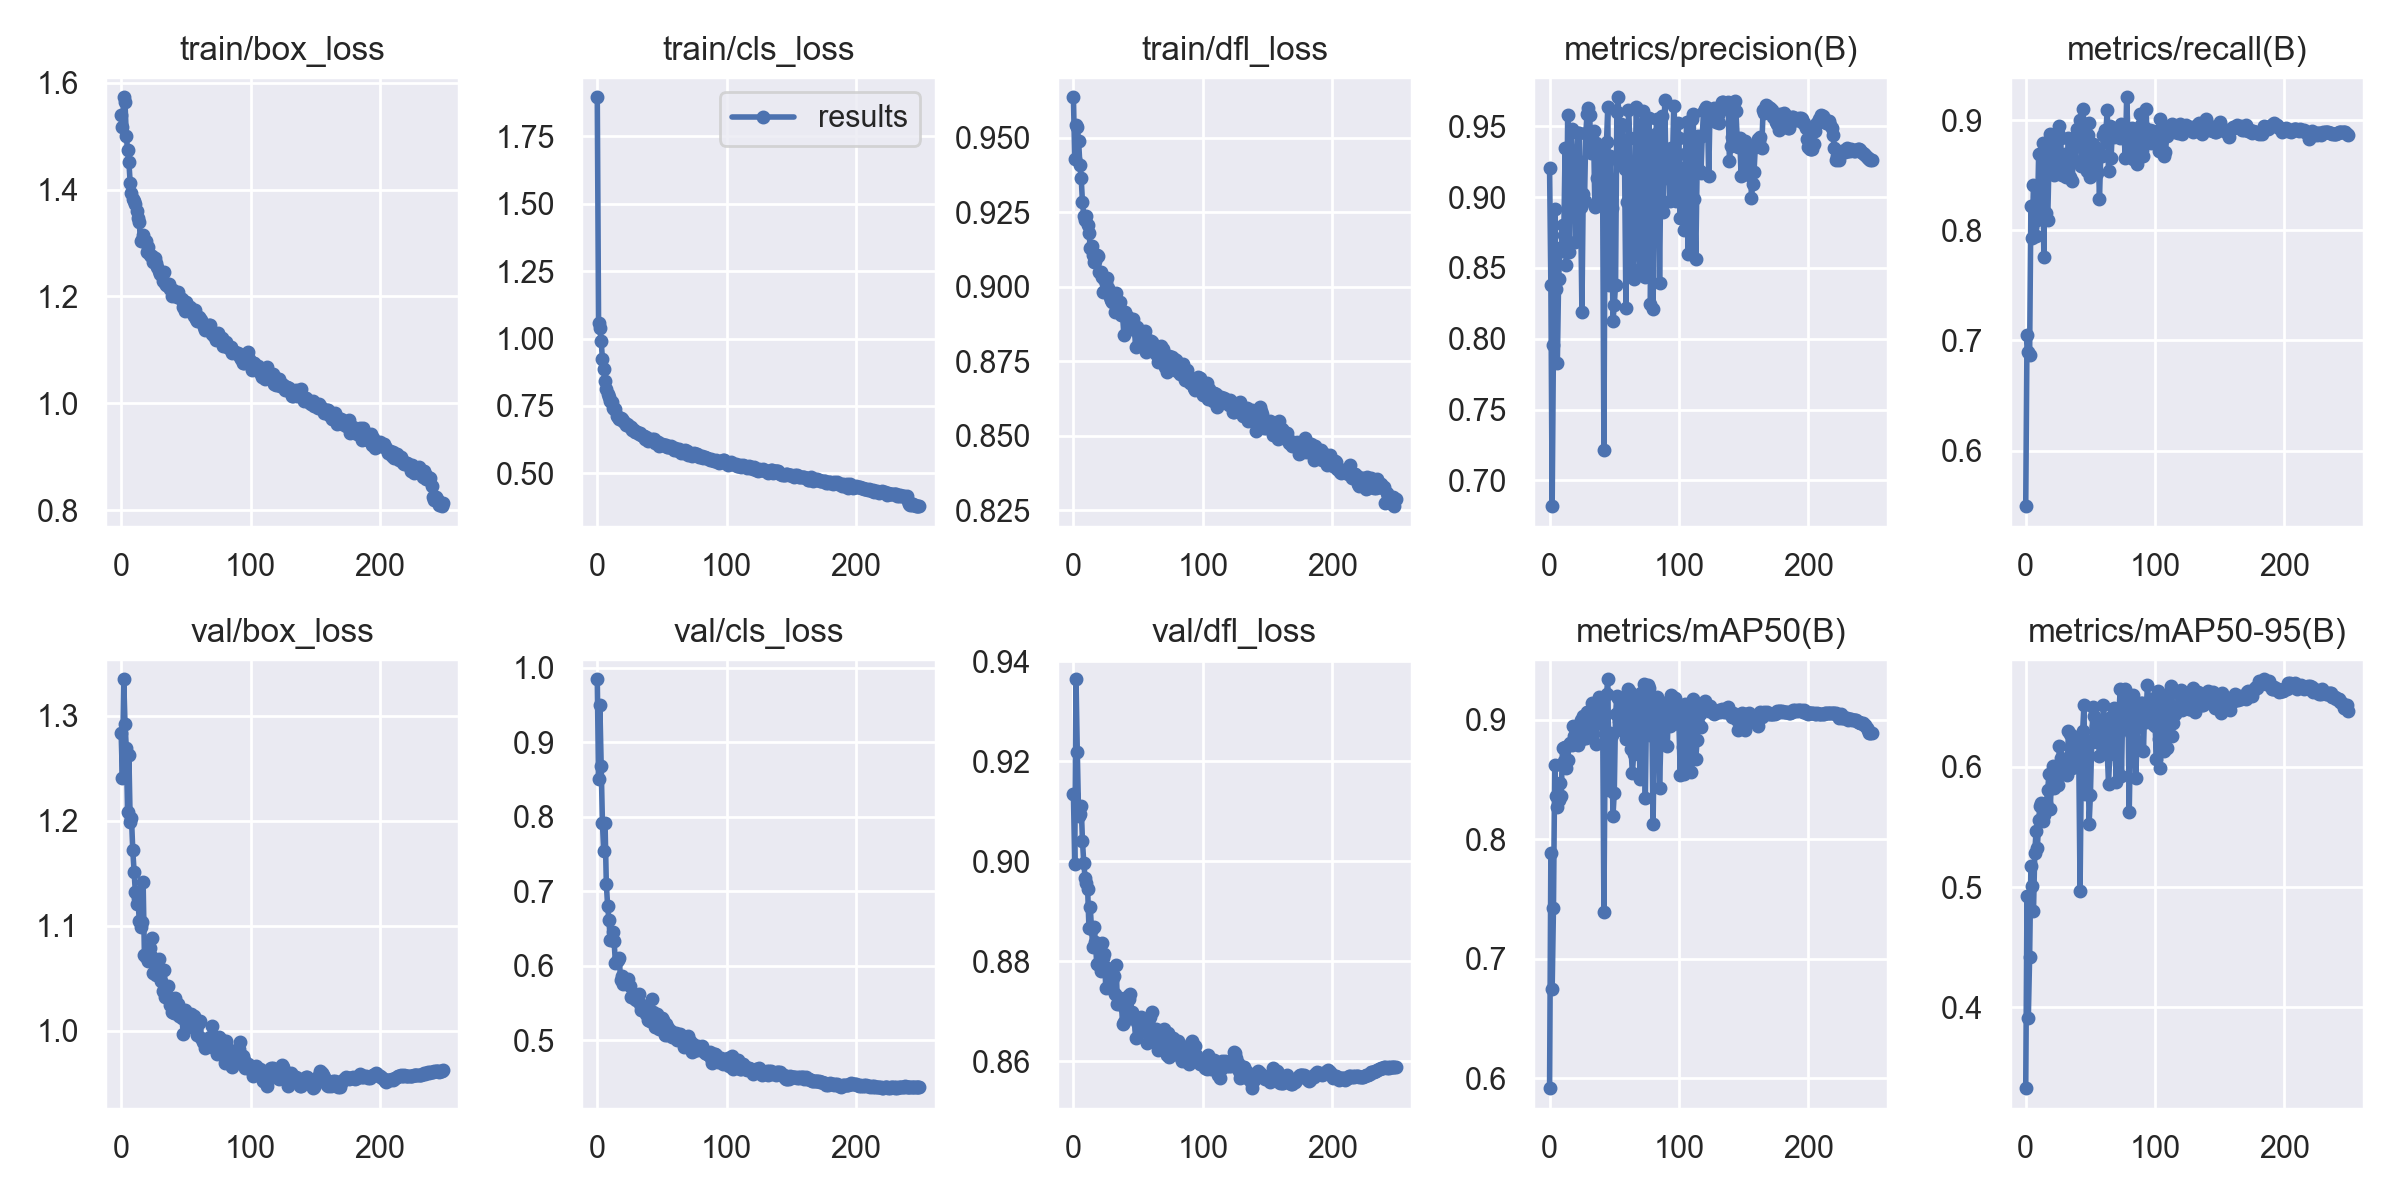
\includegraphics[scale=0.5]{bab4/grafik_model_malam.png}
  \caption{Grafik Hasil Pelatihan Model pada Malam Hari}
  \label{fig:grafik model malam}
\end{figure}

Gambar \ref{fig:grafik model malam} menunjukkan grafik-grafik hasil pelatihan model \emph{YOLOv8} yang dilatih selama 250 epoch. Grafik pertama, yaitu \emph{train/box\_loss} dan \emph{val/box\_loss}, menggambarkan \emph{bounding box loss} pada data pelatihan maupun data validasi. Kedua grafik ini menunjukkan penurunan yang stabil, yang menandakan bahwa model semakin baik dalam memprediksi posisi objek seiring dengan bertambahnya jumlah epoch. Demikian pula, grafik \emph{train/cls\_loss} dan \emph{val/cls\_loss} untuk \emph{classification loss} menunjukkan penurunan yang konsisten, menandakan bahwa model semakin akurat dalam mengklasifikasikan objek pada data pelatihan dan validasi. \emph{train/dfl\_loss} dan \emph{val/dfl\_loss} menunjukkan \emph{distribution for logits loss}, yang juga menurun dengan stabil, yang menunjukkan bahwa distribusi prediksi model semakin mendekati distribusi yang benar. Grafik \emph{metrics/precision} dan \emph{metrics/recall} menggambarkan \emph{precision} dan \emph{recall} model pada data pelatihan dan validasi. Seiring berjalannya epoch, kedua metrik ini menunjukkan peningkatan yang signifikan, dengan \emph{precision} dan \emph{recall} yang mendekati 1, menandakan bahwa model semakin efektif dalam mendeteksi objek dengan akurasi yang tinggi.

Di sisi lain, grafik \emph{metrics/mAP50} dan \emph{metrics/mAP50-95} menunjukkan \emph{mean Average Precision} (mAP) pada level IoU 0.5 dan rata-rata mAP pada interval 0.5 hingga 0.95. \emph{mAP50} menunjukkan performa deteksi model pada threshold IoU 0.5 dan terus meningkat, mencerminkan bahwa model semakin akurat dalam deteksi objek, sementara \emph{mAP50-95} menunjukkan performa model secara keseluruhan pada berbagai threshold IoU. Kedua grafik ini menunjukkan peningkatan yang stabil, meskipun terdapat sedikit fluktuasi, yang mungkin disebabkan oleh variasi dalam data validasi. Secara keseluruhan, grafik-grafik ini menunjukkan bahwa model \emph{YOLOv8} berhasil dilatih dengan baik, dengan peningkatan akurasi deteksi objek dan kemampuan model dalam mengurangi kerugian secara bertahap sepanjang 250 epoch pelatihan.

Kemudian terdapat hasil confusion matrix yang didapatkan dari hasil model pelatihan ini. Confusion matrix tersebut dapat dilihat pada Gambar .

\begin{figure} [H] \centering
  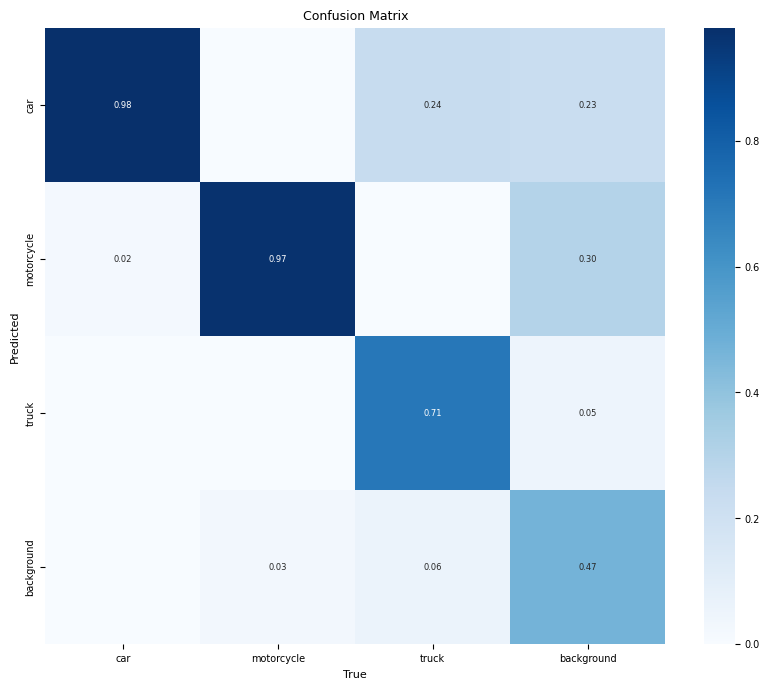
\includegraphics[scale=0.8]{bab4/confusion_malam.png}
  \caption{Confusion Matrix Model Malam Hari}
  \label{fig:confusion matrix malam}
\end{figure}
\vspace{-10pt}
Confusion matrix pada Gambar \ref{fig:confusion matrix malam} menunjukkan hasil prediksi model pada malam hari berdasarkan kategori objek yang terdeteksi.

\begin{enumerate}[nosep]
\item Kelas \emph{car}:
Model mampu mengenali objek \emph{car} dengan sangat baik, dengan tingkat keberhasilan 98\%. Meski demikian, masih ada 2\% yang keliru diklasifikasikan sebagai \emph{motorcycle}, dan 24\% lainnya salah dikenali sebagai \emph{truck}.

\item Kelas \emph{motorcycle}:  
Objek \emph{motorcycle} terdeteksi dengan akurasi 97\%, namun sebagian besar sisanya (80\%) justru salah dikira sebagai \emph{truck}. Terdapat juga sedikit kesalahan ke kelas \emph{car} (2\%) dan \emph{background} (6\%).

\item Kelas \emph{truck}:  
Model berhasil mengenali 71\% objek \emph{truck} dengan benar. Sisanya cenderung tertukar dengan \emph{motorcycle} (71\%) dan sedikit sebagai \emph{car} (3\%) atau \emph{background} (6\%).

\item Kelas \emph{background}:  
Kinerja model cukup lemah pada kelas ini, dengan hanya 3\% yang dikenali dengan benar. Beberapa bagian latar malah salah diprediksi sebagai \emph{motorcycle} (6\%), \emph{car} (6\%), dan \emph{truck} (2\%).
\end{enumerate}

Melalui analisis ini, dapat disimpulkan bahwa model \textit{YOLOv8} menunjukkan akurasi yang sangat baik dalam mendeteksi kelas \textit{car} dengan tingkat \textit{True Positive} yang sangat tinggi, sedangkan ada sedikit kesulitan dalam mendeteksi objek \textit{motorcycle} dan \textit{truck}, yang perlu diperbaiki. Selanjutnya, model perlu dioptimalkan agar lebih akurat dalam mendeteksi objek \textit{motorcycle} dan \textit{truck} dengan mengurangi \textit{False Negative} dan meningkatkan \textit{True Positive} pada kedua kelas tersebut.

Kemudian, dilakukan validasi deteksi objek dari hasil pelatihan model ini. Pada Gambar \ref{fig:validasi deteksi malam} dapat dilihat hasil model yang telah dilatih beserta \emph{confidence threshold} yang didapatkan untuk setiap citra yang digunakan sebagai validasi.

\begin{figure} [H] \centering
  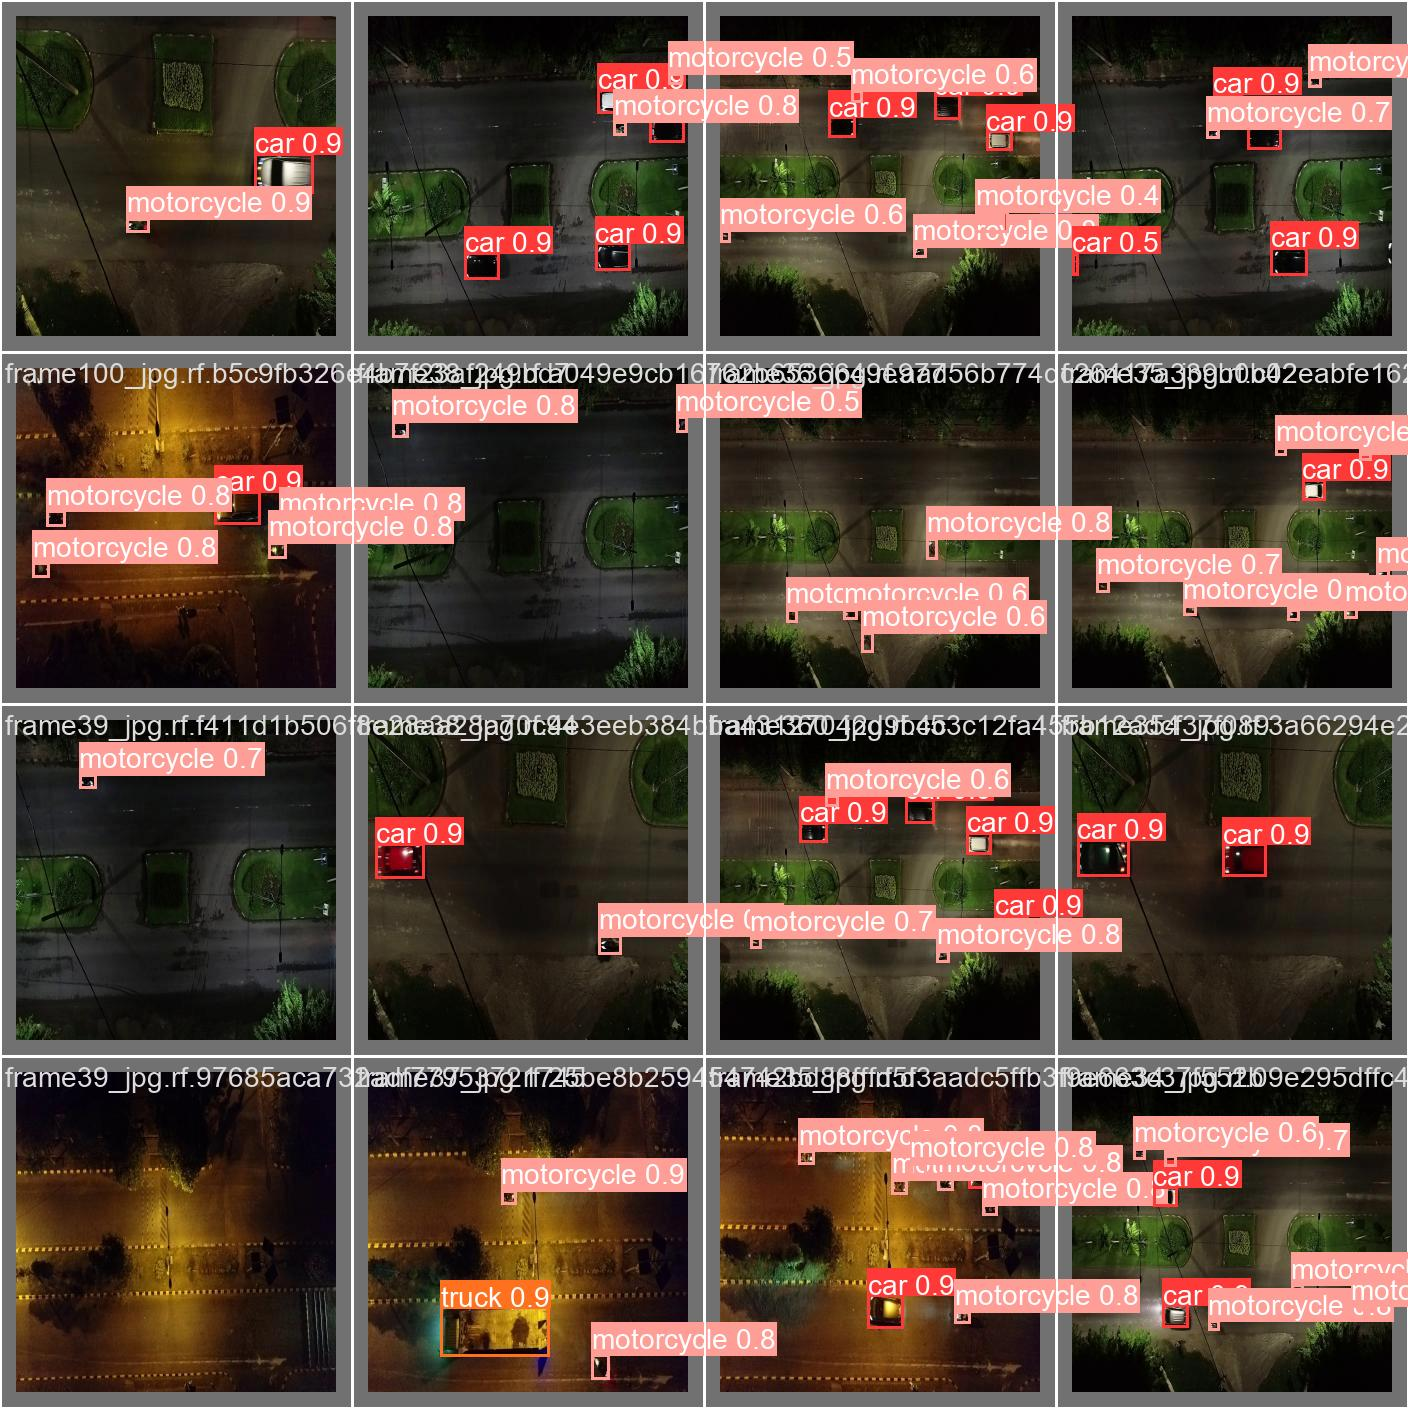
\includegraphics[scale=0.25]{bab4/val_batch_malam.jpg}
  \caption{Validasi Deteksi Malam Hari}
  \label{fig:validasi deteksi malam}
\end{figure}
\vspace{-10pt}
Dari hasil validasi deteksi tersebut objek kecil seperti motor mendapatkan nilai \emph{confidence threshold} paling kecil 0.5 dan paling tinggi 0.9. Untuk mobil rata-rata mendapatkan 0.8 hingga 0.9.

\section{Perbandingan dengan Data Penelitian Terdahulu}
Pada sub-bab ini akan dilakukan analisis terhadap pengujian yang didapatkan dari penelitian ini dan dilakukan perbandingan dengan penelitian terdahulu. Terdapat dua penelitian terdahulu yang digunakan, antara lain:
\begin{enumerate}[nosep]
  \item Perhitungan Kecepatan Kendaraan Menggunakan Drone Bergerak dengan Metode Deep Learning (Fatchurozi, 2024) \\
  \item Vehicle Tracking and Speed Estimation from Unmanned Aerial Vehicles Using Segmentation Initialised Trackers (Tilon \& Nex, 2023) \\
\end{enumerate}


\subsection{Pengujian dan Perbandingan Sistem terhadap Kecepatan Rata-rata dibawah 25km/h pada Siang Hari}
Pengujian ini dilakukan dengan kendaraan motor yang dikendarai dengan kecepatan rata-rata 20km/h dengan \emph{drone} diam. Tujuan dilakukan pengujian ini untuk mendapatkan informasi terkait kinerja terhadap sistem sejauh mana akurasi perhitungannya. Pengujian dilakukan pada siang hari dengan \emph{interval} waktu antara 11.00 WIB hingga 13.00 WIB. Pengujian dilakukan sebanyak 4 kali percobaan dengan kecepatan yang diproyeksikan sebesar 20km/h. Referensi untuk hasil sistem digunakan perhitungan manual di setiap ketinggian. Rata-rata kecepatan dari perhitungan manual ditunjukkan pada Tabel \ref{table:20km/h-siang-manual} dan Perhitungan Manual dari Penelitian \ref{subsec:Iqbal2024}. 

\begin{table}[H]
	\caption{Perhitungan Manual dengan Kecepatan Rata-rata 20km/h pada Siang Hari}
    \label{table:20km/h-siang-manual}
	\centering
	\begin{tabular}{|c|c|c|c|c|}
		\hline
		\multirow{2}{*}{\textbf{Ketinggian (Meter)}} & \multicolumn{3}{c|}{\textbf{Rata-rata Kecepatan (Km/h)}} & \multirow{2}{*}{\textbf{Rata-rata (Km/h)}} \\ \cline{2-4}
		& 1 & 2 & 3 & \\ \hline
		20 & 23,33 & 22,9 & 22,3 & 22,84 \\
		30 & 18,94 & 18,8 & 18,76 & 18,83 \\
		40 & 18,81 & 18,79 & 18,72 & 18,77 \\ \hline
	\end{tabular}
\end{table}
\vspace{-10pt}
\begin{table}[H]
	\caption{Perhitungan Manual Penelitian \ref{subsec:Iqbal2024} dengan Kecepatan Rata-rata 20km/h pada Siang Hari}
    \label{table:20km/h-siang-manual-iqbal}
	\centering
	\begin{tabular}{|c|c|c|c|c|}
		\hline
		\multirow{2}{*}{\textbf{Ketinggian (Meter)}} & \multicolumn{3}{c|}{\textbf{Rata-rata Kecepatan (Km/h)}} & \multirow{2}{*}{\textbf{Rata-rata (Km/h)}} \\ \cline{2-4}
		& 1 & 2 & 3 & \\ \hline
		20 & 19,46 & 19,71 & 19,86 & 19,67 \\
		30 & 19,31 & 18,77 & 18,93 & 19,00 \\
		40 & 19,48 & 18,81 & 18,87 & 19,05 \\ \hline
	\end{tabular}
\end{table}
\vspace{-10pt}
\begin{table}[H]
	\caption{Perhitungan Manual Penelitian \ref{subsec:Tilon2023} dengan Kecepatan Rata-rata 15 km/h}
    \label{table:15kmh-manual-Tilon}
	\centering
	\begin{tabular}{|c|c|}
		\hline
		\textbf{Ketinggian (Meter)} & \textbf{Kecepatan Aktual(Km/h)}\\ \hline
		50 & 14,68 \\ \hline
	\end{tabular}
\end{table}

Pada Tabel \ref{table:20km/h-siang-manual} yang menunjukkan hasil perhitungan manual dari penelitian ini dengan Tabel \ref{table:20km/h-siang-manual-iqbal} terdapat perbedaan di setiap ketinggiannya terutama pada ketinggian 20 meter yang memiliki selisih hingga 3km/h. Hal ini dapat disebabkan karena beberapa faktor \emph{error} yang dilakukan peneliti baik dalam mengukur jarak aktual dan waktu aktual saat objek yang menjadi objek percobaan melintas. Untuk Penelitian \ref{subsec:Tilon2023} yang ditunjukkan pada Tabel \ref{table:15kmh-manual-Tilon} memiliki kecepatan aktual yang tidak jauh dari target kecepatannya 15km/h.

Hasil pengujian terhadap sistem estimasi kecepatan yang dilakukan ditunjukkan pada Tabel \ref{table:20km/h-siang-sistem} dan dari penelitian terdahulu, yaitu Penelitian Fatchurozi \ref{subsec:Iqbal2024} pada Tabel \ref{table:20km/h-siang-iqbal}, dan Penelitian Tilon \& Nex \ref{subsec:Tilon2023} pada Tabel \ref{table:15kmh-sistem-Tilon} dapat dilihat pada Tabel \ref{table:20km/h-siang-sistem}.

Kemudian, dilakukan pengujian sistem dengan diberikan informasi tambahan, antara lain standar deviasi, dan \emph{error} antara hasil pengujian dengan perhitungan manual. Standar deviasi digunakan untuk mengetahui seberapa jauh hasil rata-rata dengan setiap data sehingga didapatkan informasi apakah tiap titik data bervariasi sangat jauh atau tidak untuk perbedaannya. Berikut persamaan yang akan digunakan untuk menghitung standar deviasi dan \emph{error} setiap data beserta akurasi yang didapatkan:

\begin{equation}
\sigma = \sqrt{\frac{\sum_{i=1}^n (x_i - \mu)^2}{n}} \label{eq:standardeviasi}
\end{equation}

Dimana:

\[
\begin{aligned}
\sigma & = \text{Standar Deviasi} \\
n & = \text{Jumlah data} \\
x_i & = \text{Data ke-i} \\
\mu & = \text{Rata-rata}
\end{aligned}
\]

Kemudian, untuk menghitung \emph{error} setiap data digunakan persamaan sebagai berikut:

\begin{equation}
\text{Error} = \text{Hasil Pengujian Sistem} - \text{Hasil Perhitungan Manual} \label{eq:error}
\end{equation}

\begin{equation}
\text{Absolute Error} = \left| \text{Error} \right| \label{eq:absolute_error}
\end{equation}

\begin{equation}
\text{Relative Error} = \left( \frac{\text{Absolute Error}}{\text{Hasil Perhitungan Manual}} \right) \times 100\% \label{eq:relative_error}
\end{equation}

Persamaan perhitungan akurasi adalah sebagai berikut:

\begin{equation}
\text{Accuracy} = 100\% - \text{Relative Error} \label{eq:accuracy}
\end{equation}

Setelah dilakukan pengujian sistem dengan kecepatan rata-rata 20km/h dan data dari penelitian terdahulu, akan dihitung seberapa akurat sistem. Berikut data hasil pengujian yang telah dilakukan beserta hasil dari penelitian terdahulu dapat dilihat pada Tabel \ref{table:20km/h-siang-sistem}, Tabel \ref{table:20km/h-siang-iqbal}, dan Tabel \ref{table:15kmh-sistem-Tilon}.

\begin{table}[H]
	\caption{Pengujian dengan Kecepatan Rata-rata 20km/h pada Siang Hari}
    \label{table:20km/h-siang-sistem}
	\centering
	\begin{tabular}{|c|c|c|c|c|c|}
		\hline
		\multirow{2}{*}{\makecell{\textbf{Ketinggian} \\ \textbf{(Meter)}}}& \multicolumn{3}{c|}{\textbf{Rata-rata Kecepatan (Km/h)}} & \multirow{2}{*}{\makecell{\textbf{Rata-rata} \\ \textbf{(Km/h)}}} & \multirow{2}{*}{\makecell{\textbf{Standar} \\ \textbf{Deviasi}}} \\ \cline{2-4}
		& 1 & 2 & 3 & \\ \hline
		20 & 21,59 & 20,06 & 21,61 & 21,09 & 0,72\\
		30 & 23,28 & 21,25 & 25,05 & 23,19 & 1,55\\
		40 & 22,24 & 24,39 & 21,7 & 22,78 & 1,16\\ \hline
	\end{tabular}
\end{table}
\vspace{-10pt}
\begin{table}[H]
	\caption{Pengujian Peneletian \ref{subsec:Iqbal2024} dengan Kecepatan Rata-rata 20km/h pada Siang Hari}
    \label{table:20km/h-siang-iqbal}
	\centering
	\begin{tabular}{|c|c|c|c|c|c|}
		\hline
		\multirow{2}{*}{\makecell{\textbf{Ketinggian} \\ \textbf{(Meter)}}} & \multicolumn{3}{c|}{\textbf{Rata-rata Kecepatan (Km/h)}} & \multirow{2}{*}{\makecell{\textbf{Rata-rata} \\ \textbf{(Km/h)}}} & \multirow{2}{*}{\makecell{\textbf{Standar} \\ \textbf{Deviasi}}} \\ \cline{2-4}
		& 1 & 2 & 3 & \\ \hline
		20 & 17,86 & 18,64 & 18,62 & 18,37 & 1,61 \\ 
		30 & 17,80 & 17,84 & 17,64 & 17,76 & 0,97 \\ 
		40 & 17,69 & 17,90 & 17,90 & 17,83 & 1,10 \\ \hline
	\end{tabular}
\end{table}
\vspace{-10pt}
\begin{table}[H]
	\caption{Pengujian Penelitian \ref{subsec:Tilon2023} dengan Kecepatan Rata-rata 15 km/h}
    \label{table:15kmh-sistem-Tilon}
	\centering
	\begin{tabular}{|c|c|}
		\hline
		\textbf{Ketinggian (Meter)} & \textbf{Kecepatan Prediksi(Km/h)} \\ \hline
		50 & 17,97 \\ \hline
	\end{tabular}
\end{table}

Hasil pengujian menunjukkan rata-rata kecepatan kendaraan antara 21,09 hingga 23,19 km/h dengan variasi terbesar pada ketinggian 30 meter. Jika dibandingkan dengan perhitungan manual yang juga menggunakan target kecepatan 20 km/h, rata-rata kecepatan manual berada di kisaran 18,77 hingga 22,84 km/h, sehingga dapat diketahui terdapat selisih antara perhitungan manual dan sistem. Dibandingkan dengan penelitian 2.1.1 yang juga menargetkan kecepatan 20 km/h, hasilnya lebih rendah, yakni sekitar 17-18 km/h dan apabila melihat perhitungan manual yang memiliki rata-rata kecepatan sekitar 19 km/h, terdapat selisih antara perhitungan manual dan sistem dengan variasi yang lebih kecil. Sementara itu, penelitian 2.1.2 yang menargetkan kecepatan 15 km/h pada ketinggian 50 meter mencatat kecepatan aktual manual 14,68 km/h dan prediksi 17,97 km/h, yang sedikit lebih tinggi dari target.

Berikut data \emph{error} dan tingkat akurasi yang didapatkan berdasarkan hasil pengujian sistem dan penelitian terdahulu:

\begin{table}[H]
\centering
\caption{Perhitungan Error dan Akurasi dengan Kecepatan Rata-rata 20Km/h saat Siang Hari pada Percobaan 1}
\label{table:error_accuracy_titik1}
\begin{tabular}{|c|c|c|c|c|}
\hline
\textbf{Ketinggian (m)} & \textbf{Error} & \textbf{Absolute Error} & \textbf{Relative Error (\%)} & \textbf{Accuracy (\%)} \\ \hline
20 & -1.74 & 1.74 & 7.46 & 92.54 \\
30 & 4.34 & 4.34 & 22.91 & 77.09 \\
40 & 3.43 & 3.43 & 18.23 & 81.77 \\ \hline
\end{tabular}
\end{table}

\begin{table}[H]
\centering
\caption{Perhitungan Error dan Akurasi Kecepatan Rata-rata 20Km/h saat Siang Hari pada Percobaan 2}
\label{table:error_accuracy_titik2}
\begin{tabular}{|c|c|c|c|c|}
\hline
\textbf{Ketinggian (m)} & \textbf{Error} & \textbf{Absolute Error} & \textbf{Relative Error (\%)} & \textbf{Accuracy (\%)} \\ \hline
20 & -2.84 & 2.84 & 12.41 & 87.59 \\
30 & 2.45 & 2.45 & 13.03 & 86.97 \\
40 & 5.60 & 5.60 & 29.79 & 70.21 \\ \hline
\end{tabular}
\end{table}

\begin{table}[H]
\centering
\caption{Perhitungan Error dan Akurasi Kecepatan Rata-rata 20Km/h saat Siang Hari pada Percobaan 3}
\label{table:error_accuracy_titik3}
\begin{tabular}{|c|c|c|c|c|}
\hline
\textbf{Ketinggian (m)} & \textbf{Error} & \textbf{Absolute Error} & \textbf{Relative Error (\%)} & \textbf{Accuracy (\%)} \\ \hline
20 & -0.69 & 0.69 & 3.10 & 96.90 \\
30 & 6.29 & 6.29 & 33.55 & 66.45 \\
40 & 2.98 & 2.98 & 15.91 & 84.09 \\ \hline
\end{tabular}
\end{table}
Tabel hasil perhitungan \emph{error} dari pengujian menunjukkan akurasi pengukuran kecepatan \emph{drone} pada tiga percobaan dan ketinggian berbeda. Percobaan 1 memiliki akurasi tertinggi 92,54\% di 20 m, turun ke 77,09\% di 30 m, lalu naik ke 81,77\% di 40 m. Percobaan 2 akurasinya terbaik 87,59\% di 20 m dan terendah 70,21\% di 40 m. Percobaan 3 mencatat akurasi tertinggi 96,90\% di 20 m dan terendah 66,45\% di 30 m. Secara keseluruhan, ketinggian 20 meter cenderung memberikan hasil pengukuran paling akurat dan konsisten.

\begin{table}[H]
\centering
\caption{Akurasi pada Penelitian \ref{subsec:Iqbal2024} dengan Kecepatan Rata-rata 20 km/h saat Siang Hari}
\label{table:accuracy_iqbal}
\begin{tabular}{|c|c|c|c|}
\hline
\textbf{Ketinggian (m)} & \textbf{Percobaan 1 (\%)} & \textbf{Percobaan 2 (\%)} & \textbf{Percobaan 3 (\%)} \\ \hline
20 & 89.75 & 90.52 & 88.26 \\
30 & 93.47 & 91.55 & 87.98 \\
40 & 86.11 & 94.96 & 89.13 \\ \hline
\end{tabular}
\end{table}

\begin{table}[H]
\centering
\caption{Akurasi pada Penelitian \ref{subsec:Tilon2023} dengan Kecepatan Rata-rata 15 km/h}
\label{table:accuracy_tilon}
\begin{tabular}{|c|c|}
\hline
\textbf{Ketinggian (m)} & \textbf{Percobaan 1 (\%)} \\ \hline
50 & 77,59 \\ \hline
\end{tabular}
\end{table}

Berdasarkan hasil pengujian yang dilakukan beserta perbandingan dengan data penelitian terdahulu, beberapa hal yang dapat disimpulkan terkait akurasi pengukuran kecepatan kendaraan menggunakan drone adalah sebagai berikut:

\begin{itemize}[nolistsep]
    \item Tabel 4.9 dan 4.11 menunjukkan akurasi pengukuran \emph{drone} pada tiga percobaan dan ketinggian 20, 30, dan 40 meter.
    \item Percobaan 1 mencatat akurasi:
    \begin{itemize}[nolistsep]
        \item Tertinggi 92,54\% pada 20 m,
        \item Turun ke 77,09\% di 30 m,
        \item Naik ke 81,77\% di 40 m.
    \end{itemize}
    \item Percobaan 2 menunjukkan akurasi relatif stabil dengan:
    \begin{itemize}[nolistsep]
        \item Puncak 87,59\% pada 20 m,
        \item Terendah 70,21\% pada 40 m.
    \end{itemize}
    \item Percobaan 3 memiliki variasi akurasi terbesar, yaitu:
    \begin{itemize}[nolistsep]
        \item 96,90\% di 20 m,
        \item Turun tajam ke 66,45\% di 30 m,
        \item Naik ke 84,09\% di 40 m.
    \end{itemize}
    \item Secara keseluruhan, ketinggian 20 meter memberikan hasil pengukuran yang paling akurat dan konsisten.
    \item Penelitian 2.1.1 (kecepatan rata-rata 20 km/h) menunjukkan akurasi yang lebih konsisten dan tinggi, berkisar dari 87\% hingga 89,13\%, dibandingkan penelitian ini.
    \item Penelitian 2.1.2 (kecepatan 15 km/h, ketinggian 50 m) memiliki akurasi lebih rendah (77,59\%), menunjukkan pengaruh kecepatan dan ketinggian pada akurasi.
    \item Faktor lain yang penting diperhatikan untuk meningkatkan akurasi meliputi:
    \begin{itemize}[nolistsep]
        \item Getaran drone,
        \item Kondisi cuaca,
        \item Kestabilan \emph{device}.
        \item Pengaturan kecepatan kendaraan
    \end{itemize}
\end{itemize}
Sehingga, hasil pengujian sistem pada penelitian ini dengan penelitian terdahulu tentu memiliki perbedaan yang disebabkan penggunaan atau kondisi lingkungan yang berbeda.
\vspace{20pt}
\section{Pengujian dan Perbandingan Sistem terhadap Kecepatan Rata-rata diatas 25Km/h pada Siang Hari}
Pengujian ini dilakukan dengan kecepatan rata-rata 40km/h pada siang hari dengan \emph{drone} diam dan pada waktu antara 12.00 WIB hingga 14.00 WIB. Sebanyak 4 kali percobaan dilakukan untuk mendapatkan data pengujian. Perhitungan manual digunakan sebagai referensi dari perhitungan sistem. Perhitungan Manual untuk kecepatan rata-rata 40km/h pada siang hari dapat dilihat pada Tabel \ref{table:40km/h-siang-manual} hingga Tabel \ref{table:30kmh-manual-Tilon}.

\begin{table}[H]
	\caption{Perhitungan Manual dengan Kecepatan Rata-rata 40km/h pada Siang Hari}
    \label{table:40km/h-siang-manual}
	\centering
	\begin{tabular}{|c|c|c|c|c|}
		\hline
		\multirow{2}{*}{\textbf{Ketinggian (Meter)}} & \multicolumn{3}{c|}{\textbf{Rata-rata Kecepatan (Km/h)}} & \multirow{2}{*}{\textbf{Rata-rata (Km/h)}} \\ \cline{2-4}
		& 1 & 2 & 3 & \\ \hline
		20 & 39,8 & 39,24 & 39,4 & 39,48 \\
		30 & 39,62 & 39,57 & 38,52 & 39,23 \\
		40 & 39,88 & 39,94 & 39,64 & 39,82 \\ \hline
	\end{tabular}
\end{table}
\vspace{-10pt}
\begin{table}[H]
	\caption{Perhitungan Manual Penelitian \ref{subsec:Iqbal2024} dengan Kecepatan Rata-rata 40km/h pada Siang Hari}
    \label{table:40km/h-siang-manual-iqbal}
	\centering
	\begin{tabular}{|c|c|c|c|c|}
		\hline
		\multirow{2}{*}{\textbf{Ketinggian (Meter)}} & \multicolumn{3}{c|}{\textbf{Rata-rata Kecepatan (Km/h)}} & \multirow{2}{*}{\textbf{Rata-rata (Km/h)}} \\ \cline{2-4}
		& 1 & 2 & 3 & \\ \hline
		20 & 39,45 & 40,91 & 39,78 & 40,05 \\
		30 & 38,48 & 39,63 & 38,85 & 38,98 \\
		40 & 38,20 & 38,05 & 37,00 & 37,75 \\ \hline
	\end{tabular}
\end{table}
\vspace{-10pt}
\begin{table}[H]
	\caption{Perhitungan Manual Penelitian \ref{subsec:Tilon2023} dengan Kecepatan Rata-rata 30 km/h}
    \label{table:30kmh-manual-Tilon}
	\centering
	\begin{tabular}{|c|c|}
		\hline
		\textbf{Ketinggian (Meter)} & \textbf{Kecepatan Aktual(Km/h)}\\ \hline
		50 & 28,55 \\ \hline
	\end{tabular}
\end{table}

Pada Tabel \ref{table:40km/h-siang-manual} terlihat perhitungan manual pada target kecepatan 40 km/h menghasilkan nilai rata-rata yang relatif rapat, yaitu 39,48 km/h pada 20 m, 39,23 km/h pada 30 m, dan 39,82 km/h pada 40 m. Selisih kurang dari 1 km/h ini mengindikasikan bahwa prosedur pengukuran jarak dan waktu cukup stabil.. Sebaliknya, pada Tabel \ref{table:40km/h-siang-manual-iqbal} (Penelitian \ref{subsec:Iqbal2024}) variasi tiap ketinggian meluas terutama di 40 m, dengan deviasi hampir 2,25 km/h dari target menunjukkan peningkatan potensi \emph{error} sistematis, yang mungkin terjadi kesalahan saat pencatatan waktu kendaraan berpindah dari \emph{start} ke \emph{finish}.

Sementara itu, pada Tabel \ref{table:30kmh-manual-Tilon} (Penelitian \ref{subsec:Tilon2023}) dengan target 30 km/h pada ketinggian 50 m diperoleh kecepatan aktual 28,55 km/h, alias selisih 1,45 km/h. Meskipun nilai absolut error lebih kecil dibandingkan variasi di Penelitian \ref{subsec:Iqbal2024}, perbedaan ini masih menunjukkan bahwa tanpa analisis statistik lebih lanjut dan kurangnya informasi pengambilan datanya, tidak mudah untuk mengetahui perbedaan tersebut.

Kemudian, didapatkan data pengujian sistem dengan kecepatan rata-rata 40km/h, beserta data dari penelitian terdahulu sehingga dapat diketahui seberapa akurat sistem. Hasil data pengujian dan data penelitian terdahulu dapat dilihat pada Tabel \ref{table:40km/h-siang-sistem}, Tabel \ref{table:40km/h-siang-iqbal}, dan Tabel \ref{table:30kmh-sistem-Tilon}.

\begin{table}[H]
	\caption{Pengujian dengan Kecepatan Rata-rata 40km/h pada Siang Hari}
    \label{table:40km/h-siang-sistem}
	\centering
	\begin{tabular}{|c|c|c|c|c|c|}
		\hline
		\multirow{2}{*}{\makecell{\textbf{Ketinggian} \\ \textbf{(Km/h)}}}& \multicolumn{3}{c|}{\textbf{Rata-rata Kecepatan (Km/h)}} & \multirow{2}{*}{\makecell{\textbf{Rata-rata} \\ \textbf{(Km/h)}}} & \multirow{2}{*}{\makecell{\textbf{Standar} \\ \textbf{Deviasi}}} \\ \cline{2-4}
		& 1 & 2 & 3 & \\ \hline
		20 & 37,8 & 36,5 & 43,6 & 39,3 & 3,09\\
		30 & 37,64 & 37,35 & 35,35 & 36,78 & 1,01\\
		40 & 36,58 & 36,64 & 35 & 36,07 & 0,76\\ \hline
	\end{tabular}
\end{table}
\vspace{-10pt}
\begin{table}[H]
	\caption{Pengujian Peneletian \ref{subsec:Iqbal2024} dengan Kecepatan Rata-rata 40km/h pada Siang Hari}
    \label{table:40km/h-siang-iqbal}
	\centering
	\begin{tabular}{|c|c|c|c|c|c|}
		\hline
		\multirow{2}{*}{\makecell{\textbf{Ketinggian} \\ \textbf{(Meter)}}} & \multicolumn{3}{c|}{\textbf{Rata-rata Kecepatan (Km/h)}} & \multirow{2}{*}{\makecell{\textbf{Rata-rata} \\ \textbf{(Km/h)}}} & \multirow{2}{*}{\makecell{\textbf{Standar} \\ \textbf{Deviasi}}} \\ \cline{2-4}
		& 1 & 2 & 3 & \\ \hline
		20 & 35,40 & 37,03 & 35,11 & 35,85 & 1,91 \\ 
		30 & 35,97 & 36,28 & 34,18 & 35,47 & 3,04 \\ 
		40 & 32,89 & 36,13 & 32,98 & 34,00 & 2,50 \\ \hline
	\end{tabular}
\end{table}
\vspace{-10pt}
\begin{table}[H]
	\caption{Pengujian Penelitian \ref{subsec:Tilon2023} dengan Kecepatan Rata-rata 30 km/h}
    \label{table:30kmh-sistem-Tilon}
	\centering
	\begin{tabular}{|c|c|}
		\hline
		\textbf{Ketinggian (Meter)} & \textbf{Kecepatan Prediksi(Km/h)} \\ \hline
		50 & 22,83 \\ \hline
	\end{tabular}
\end{table}

Hasil pengujian pada Tabel \ref{table:40km/h-siang-sistem} menunjukkan standar deviasi tertinggi pada ketinggian 20m sebesar (3.09) yang menandakan terdapat variasi rata-rata dari kecepatan yang dihitung di semua percobaan. Kemudian, pada Penelitian \ref{table:40km/h-siang-iqbal} menunjukkan standar deviasi tertinggi pada ketinggian 30m sebesar (3.04). Apabila dilihat antara hasil pengujian sistem dengan penelitian terdahulu mengalami beberapa variasi dan terdapat \emph{error}, seperti pada Tabel \ref{table:30kmh-sistem-Tilon} terlihat selisih kecepatan hasil pengujiannya dengan hasil perhitungan manual pada Tabel \ref{table:30kmh-manual-Tilon} sekitar 6km/h.

Setelah didapatkan data hasil pengujian, dapat dihitung seberapa besar \emph{error} yang dialami dan tingkat akurasi masing-masing sistem.

\begin{table}[H]
\centering
	\caption{Perhitungan Error dan Akurasi dengan Kecepatan Rata-rata 40Km/h saat Siang Hari pada Percobaan 1}
	\label{table:error_accuracy_per1_40km/h_siang}
	\begin{tabular}{|c|c|c|c|c|}
	\hline
	\textbf{Ketinggian (m)} & \textbf{Error} & \textbf{Absolute Error} & \textbf{Relative Error (\%)} & \textbf{Accuracy (\%)} \\
	\hline
	20 & -2.00 & 2.00 & 5.03 & 94.97 \\
	30 & -1.98 & 1.98 & 5.00 & 95.00 \\
	40 & -3.30 & 3.30 & 8.28 & 91.72 \\
	\hline
	\end{tabular}
\end{table}
\vspace{-10pt}
\begin{table}[H]
\centering
	\caption{Perhitungan Error dan Akurasi dengan Kecepatan Rata-rata 40Km/h saat Siang Hari pada Percobaan 2}
	\label{table:error_accuracy_per2_40km/h_siang}
	\begin{tabular}{|c|c|c|c|c|}
	\hline
	\textbf{Ketinggian (m)} & \textbf{Error} & \textbf{Absolute Error} & \textbf{Relative Error (\%)} & \textbf{Accuracy (\%)} \\
	\hline
	20 & -2.74 & 2.74 & 6.98 & 93.02 \\
	30 & -2.22 & 2.22 & 5.61 & 94.39 \\
	40 & -3.30 & 3.30 & 8.27 & 91.73 \\
	\hline
	\end{tabular}
\end{table}
\vspace{-10pt}
\begin{table}[H]
\centering
	\caption{Perhitungan Error dan Akurasi dengan Kecepatan Rata-rata 40Km/h saat Siang Hari pada Percobaan 3}
	\label{table:error_accuracy_per3_40km/h_siang}
	\begin{tabular}{|c|c|c|c|c|}
	\hline
	\textbf{Ketinggian (m)} & \textbf{Error} & \textbf{Absolute Error} & \textbf{Relative Error (\%)} & \textbf{Accuracy (\%)} \\
	\hline
	20 & 4.20 & 4.20 & 10.66 & 89.34 \\
	30 & -3.17 & 3.17 & 8.23 & 91.77 \\
	40 & -4.64 & 4.64 & 11.71 & 88.29 \\
	\hline
	\end{tabular}
\end{table}
\vspace{-10pt}
Berdasarkan ketiga tabel tersebut dapat dilihat bahwa pada Percobaan 1 (Tabel \ref{table:error_accuracy_per1_40km/h_siang}) nilai \emph{error} berkisar antara –3,30 hingga –2,00 km/h dengan relative \emph{error} tertinggi 8,28\% (pada ketinggian 40 m) dan akurasi minimal 91,72\%. Pada Percobaan 2 (Tabel \ref{table:error_accuracy_per2_40km/h_siang}) memiliki \emph{error} di sekitar –3,30 hingga –2,22 km/h, dan \emph{relative error} tertinggi 8,27\% sehingga akurasi minimal 91,73\%. Sedangkan pada Percobaan 3 (Tabel \ref{table:error_accuracy_per3_40km/h_siang}) terlihat \emph{error} paling variatif, dari 4,20 km/h pada ketinggian 20m hingga –4,64 km/h pada 40m, dengan \emph{relative error} tertinggi 11,71\% dan akurasi terendah 88,29\%. Secara umum, semakin besar ketinggian, semakin besar deviasi hasil sistem terhadap hitungan manual, dan Percobaan 3 menunjukkan fluktuasi error paling signifikan dibanding dua percobaan sebelumnya, yang mengindikasikan kondisi pengukuran, misalnya pencahayaan atau sudut pandang \emph{drone} paling tidak stabil pada saat percobaan ketiga.

\begin{table}[H]
\centering
	\caption{Akurasi pada Penelitian \ref{subsec:Iqbal2024} dengan Kecepatan Rata-rata 40 Km/h saat Siang Hari}
	\label{table:accuracy_40km/h_iqbal}
	\begin{tabular}{|c|c|c|c|}
	\hline
	\textbf{Ketinggian (m)} & \textbf{Percobaan 1 (\%)} & \textbf{Percobaan 2 (\%)} & \textbf{Percobaan 3 (\%)} \\
	\hline
	20 & 89,75 & 90,52 & 88,26 \\
	30 & 93,47 & 91,55 & 87,98 \\
	40 & 86,11 & 94,96 & 89,13 \\
	\hline
	\end{tabular}
\end{table}
\vspace{-10pt}
\begin{table}[H]
\centering
\caption{Akurasi pada Penelitian \ref{subsec:Tilon2023} dengan Kecepatan Rata-rata 30 km/h}
\label{table:accuracy_tilon_30km/h}
\begin{tabular}{|c|c|}
\hline
\textbf{Ketinggian (m)} & \textbf{Percobaan 1 (\%)} \\ \hline
50 & 79,97 \\ \hline
\end{tabular}
\end{table}

Berdasarkan hasil pengujian yang dilakukan serta perbandingan dengan data penelitian terdahulu, beberapa hal yang dapat disimpulkan terkait akurasi pengukuran kecepatan kendaraan menggunakan drone dengan kecepatan rata-rata 40\,km/h pada siang hari adalah sebagai berikut:

\begin{itemize}[nolistsep]
  \item Percobaan 1 mencatat akurasi:
    \begin{itemize}[nolistsep]
      \item Memulai pada 94,97\% di 20\,m,
      \item Meningkat ke puncak 95,05\% di 30\,m,
      \item Menurun menjadi 91,72\% di 40\,m.
    \end{itemize}
  \item Percobaan 2 menunjukkan akurasi relatif stabil dengan:
    \begin{itemize}[nolistsep]
      \item Puncak 94,39\% pada 30\,m,
      \item Terendah 91,73\% pada 40\,m.
    \end{itemize}
  \item Percobaan 3 memiliki variasi akurasi terbesar, yaitu:
    \begin{itemize}[nolistsep]
      \item Memulai pada 89,34\% di 20\,m,
      \item Meningkat ke 91,77\% di 30\,m,
      \item Menurun ke terendah 88,29\% di 40\,m.
    \end{itemize}

  \item Secara keseluruhan, ketinggian 30\,m memberikan hasil pengukuran yang paling akurat dan konsisten pada kecepatan 40\,km/h.

  \item Perbandingan dengan Penelitian Terdahulu
	\begin{itemize}[nolistsep]
	\item Penelitian \ref{subsec:Iqbal2024} (kecepatan rata-rata 40km/h) menunjukkan akurasi berkisar antara 87,98\% hingga 89,13\%, sedikit lebih rendah dan dengan variasi yang lebih besar dibandingkan penelitian ini.
	\item Penelitian \ref{subsec:Tilon2023} (kecepatan rata-rata 30km/h pada ketinggian 50m) hanya mencapai akurasi 79,97\%, menegaskan pengaruh ketinggian dan kecepatan terhadap akurasi.
	\end{itemize}
	\item Beberapa faktor penting yang perlu dipertimbangkan untuk meningkatkan akurasi pengukuran:
	\begin{itemize}[nolistsep]
	\item Perbedaan pengaturan kamera \emph{drone}
	\item Kondisi cuaca
	\item Stabilitas perangkat (device)
	\item Pengaturan kecepatan kendaraan
	\end{itemize}
\end{itemize}
Meskipun yang dilakukan penelitian objek yang sama dan fokus yang sama tetapi terdapat perbedaan hasil dikarenakan kurang sempurnanya sistem dan perbedaan perhitungan yang dilakukan.

\section{Pengujian Sistem terhadap Kecepatan Rata-rata 20Km/H pada Malam Hari}

Pada pengujian malam hari tepatnya sekitar pukul 00.30 WIB hingga 03.00 WIB, kendaraan motor dikendarai dengan kecepatan rata-rata 20 km/h. Tujuan pengujian ini adalah untuk menguji kinerja sistem pada kondisi pencahayaan yang lebih rendah dan intensitas lalu lintas yang berbeda dibandingkan dengan siang hari. Pengujian dilakukan pada malam hari untuk mengetahui sejauh mana sistem dapat mengestimasi kecepatan dalam kondisi pencahayaan yang terbatas, yang seringkali mengarah pada tantangan lebih besar dalam pengolahan citra dan deteksi objek.
\vspace{-10pt}
\begin{table}[H]
	\caption{Perhitungan Manual dengan Kecepatan Rata-rata 20km/h pada Malam Hari}
    \label{table:20km/h-malam-manual}
	\centering
	\begin{tabular}{|c|c|c|c|c|}
		\hline
		\multirow{2}{*}{\textbf{Ketinggian (Meter)}} & \multicolumn{3}{c|}{\textbf{Rata-rata Kecepatan (Km/h)}} & \multirow{2}{*}{\textbf{Rata-rata (Km/h)}} \\ \cline{2-4}
		& 1 & 2 & 3 & \\ \hline
		20 & 18,82 & 18,68 & 18,75 & 18,75 \\
		30 & 22,45 & 22,28 & 22,52 & 22,42 \\
		40 & 18,97 & 18,73 & 18,59 & 18,76 \\ \hline
	\end{tabular}
\end{table}
\vspace{-10pt}
Pada Tabel \ref{table:20km/h-malam-manual} dapat dilihat perhitungan manual dengan target kecepatan 20km/h yang menghasilkan nilai rata-rata untuk setiap ketinggiannya. Pada ketinggian 30m, terdapat perbedaan yang signifikan dengan ketinggian yang lain, dimana terukur hingga 22,42 km/h untuk rata-ratanya. Hal ini kemungkinan disebabkan karena kesalahan penguji dalam mengukur waktu dan jarak secara benar, karena semua percobaan tersebut tidak semuanya dilakukan pada hari yang sama.

\begin{table}[H]
	\caption{Pengujian dengan Kecepatan Rata-rata 20km/h pada Malam Hari}
    \label{table:20km/h-malam-sistem}
	\centering
	\begin{tabular}{|c|c|c|c|c|c|}
		\hline
		\multirow{2}{*}{\makecell{\textbf{Ketinggian} \\ \textbf{(Meter)}}}& \multicolumn{3}{c|}{\textbf{Rata-rata Kecepatan (Km/h)}} & \multirow{2}{*}{\makecell{\textbf{Rata-rata} \\ \textbf{(Km/h)}}} & \multirow{2}{*}{\makecell{\textbf{Standar} \\ \textbf{Deviasi}}} \\ \cline{2-4}
		& 1 & 2 & 3 & \\ \hline
		20 & 17,01 & 20,69 & 18,16 & 18,62 & 1,88\\
		30 & 20,88 & 23,17 & 21,32 & 21,79 & 1,22\\
		40 & 24,02 & 22,63 & 21,63 & 22,76 & 1,20\\ \hline
	\end{tabular}
\end{table}
\vspace{-10pt}
Pada Tabel \ref{table:20km/h-malam-sistem} terlihat bahwa semua ketinggian memiliki standar deviasi lebih dari nilai 1. Ketinggian 20 meter memiliki standar deviasi paling tinggi yaitu sebesar 1,88 yang menandakan variasi hasil perhitungan. Ketinggian 40 meter memiliki standar deviasi paling rendah yaitu 1,22 sedangkan ketinggian 30 meter hanya selisih 0,02 daripada ketinggian 40 meter.

Kemudian, dilakukan perhitungan \emph{error} dari hasil pengujian yang telah dilakukan untuk mengetahui seberapa akurat sistem melakukan tugasnya. Perhitungan ini dapat dilihat pada Tabel \ref{tab:20kmh-malam-p1}, \ref{tab:20kmh-malam-p2}, \ref{tab:20kmh-malam-p3}.

\begin{table}[H]
  \caption{Perhitungan Error dan Akurasi dengan Kecepatan Rata-rata 20 km/h saat Malam Hari pada Percobaan 1}
  \label{tab:20kmh-malam-p1}
  \centering
  \begin{tabular}{|c|c|c|c|c|}
    \hline
    \textbf{Ketinggian (m)} & \textbf{Error} & \textbf{Absolute Error} & \textbf{Relative Error (\%)} & \textbf{Accuracy (\%)} \\
    \hline
    20 & \(-1.81\) & 1.81 & 9.62 & 90.38 \\
    30 & \(-1.57\) & 1.57 & 6.99 & 93.01 \\
    40 &  5.05     & 5.05 & 26.63 & 73.37 \\
    \hline
  \end{tabular}
\end{table}
\vspace{-10pt}
\begin{table}[H]
  \caption{Perhitungan Error dan Akurasi dengan Kecepatan Rata-rata 20 km/h saat Malam Hari pada Percobaan 2}
  \label{tab:20kmh-malam-p2}
  \centering
  \begin{tabular}{|c|c|c|c|c|}
    \hline
    \textbf{Ketinggian (m)} & \textbf{Error} & \textbf{Absolute Error} & \textbf{Relative Error (\%)} & \textbf{Accuracy (\%)} \\
    \hline
    20 &  2.01 & 2.01 & 10.77 & 89.23 \\
    30 &  0.89 & 0.89 &  3.99 & 96.01 \\
    40 &  3.90 & 3.90 & 20.83 & 79.17 \\
    \hline
  \end{tabular}
\end{table}
\vspace{-10pt}
\begin{table}[H]
  \caption{Perhitungan Error dan Akurasi dengan Kecepatan Rata-rata 20 km/h saat Malam Hari pada Percobaan 3}
  \label{tab:20kmh-malam-p3}
  \centering
  \begin{tabular}{|c|c|c|c|c|}
    \hline
    \textbf{Ketinggian (m)} & \textbf{Error} & \textbf{Absolute Error} & \textbf{Relative Error (\%)} & \textbf{Accuracy (\%)} \\
    \hline
    20 & \(-0.59\) & 0.59 & 3.15 & 96.85 \\
    30 & \(-1.20\) & 1.20 & 5.33 & 94.67 \\
    40 &  3.04     & 3.04 & 16.36 & 83.64 \\
    \hline
  \end{tabular}
\end{table}

\section{Pengujian Sistem terhadap Kecepatan Rata-rata 40Km/H pada Malam Hari}

Selain pengujian siang hari dengan kecepatan tinggi, pengujian juga dilakukan pada malam hari sekitar pukul 00.30 WIB hingga 03.00 WIB dengan kecepatan kendaraan motor rata-rata 40 km/h. Pengujian ini bertujuan untuk mengevaluasi seberapa baik sistem dapat menangani estimasi kecepatan kendaraan yang lebih cepat meskipun dalam kondisi malam hari dengan pencahayaan yang kurang optimal. Hal ini memberikan gambaran seberapa efektif sistem bekerja di berbagai kondisi, termasuk pada malam hari dengan kecepatan tinggi, yang biasanya membutuhkan performa sistem yang lebih baik dalam mendeteksi dan menghitung kecepatan.

\begin{table}[H]
	\caption{Perhitungan Manual dengan Kecepatan Rata-rata 40km/h pada Malam Hari}
    \label{table:40km/h-malam-manual}
	\centering
	\begin{tabular}{|c|c|c|c|c|}
		\hline
		\multirow{2}{*}{\textbf{Ketinggian (Meter)}} & \multicolumn{3}{c|}{\textbf{Rata-rata Kecepatan (Km/h)}} & \multirow{2}{*}{\textbf{Rata-rata (Km/h)}} \\ \cline{2-4}
		& 1 & 2 & 3 & \\ \hline
		20 & 38,76 & 37,90 & 38,53 & 38,39 \\
		30 & 38,2 & 43,67 & 41,23 & 41,03 \\
		40 & 41,92 & 39,67 & 39,64 & 40,41 \\ \hline
	\end{tabular}
\end{table}
\vspace{-10pt}

Pada Tabel \ref{table:40km/h-malam-manual} dapat diketahui hasil perhitungan manual yang digunakan sebagai referensi dalam menentukan akurasi sistem. Pada Tabel \ref{table:40km/h-malam-sistem} akan ditampilkan hasil pengujian yang telah dilakukan.

\begin{table}[H]
	\caption{Pengujian dengan Kecepatan Rata-rata 40km/h pada Malam Hari}
    \label{table:40km/h-malam-sistem}
	\centering
	\begin{tabular}{|c|c|c|c|c|c|}
		\hline
		\multirow{2}{*}{\makecell{\textbf{Ketinggian} \\ \textbf{(Meter)}}}& \multicolumn{3}{c|}{\textbf{Rata-rata Kecepatan (Km/h)}} & \multirow{2}{*}{\makecell{\textbf{Rata-rata} \\ \textbf{(Km/h)}}} & \multirow{2}{*}{\makecell{\textbf{Standar} \\ \textbf{Deviasi}}} \\ \cline{2-4}
		& 1 & 2 & 3 & \\ \hline
		20 & 39,05 & 38,07 & 45,34 & 40,82 & 3,95 \\
		30 & 40,06 & 33,07 & 33,85 & 35,66 & 3,83 \\
		40 & 40,87 & 38,43 & 42,13 & 40,47 & 1,88 \\ \hline
	\end{tabular}
\end{table}
\vspace{-10pt}

Pada Tabel \ref{table:40km/h-malam-sistem} didapatkan standar deviasi untuk masing-masing ketinggian, yaitu 20m, 30m, dan 40m dengan kecepatan rata-rata 40km/h. Pada ketinggian 20m mengalami variasi rata-rata kecepatan yang variatif sebesar 3,95. Untuk standar deviasi terendah ada di ketinggian 40m sebesar 1,88. Untuk ketinggian 20m dan 30m terdapat selisih sebesar 0,12 dalam standar deviasi yang dimiliki.

Setelah didapatkan hasil pengujian untuk kecepatan rata-rata 40km/h tersebut maka dapat dihitung \emph{error} untuk masing-masing percobaan dan mengetahui seberapa akurasi alat ini.

\begin{table}[H]
  \caption{Perhitungan Error dan Akurasi dengan Kecepatan Rata-rata 40 km/h saat Malam Hari pada Percobaan 1}
  \label{tab:40kmh-malam-p1}
  \centering
  \begin{tabular}{|c|c|c|c|c|}
    \hline
    \textbf{Ketinggian (m)} & \textbf{Error} & \textbf{Absolute Error} & \textbf{Relative Error (\%)} & \textbf{Accuracy (\%)} \\
    \hline
    20 & 0.29  & 0.29 & 0.75 & 99.25 \\
    30 & 1.86  & 1.86 & 4.87 & 95.13 \\
    40 & \(-1.05\) & 1.05 & 2.50 & 97.50 \\
    \hline
  \end{tabular}
\end{table}
\vspace{-10pt}
\begin{table}[H]
  \caption{Perhitungan Error dan Akurasi dengan Kecepatan Rata-rata 40 km/h saat Malam Hari pada Percobaan 2}
  \label{tab:40kmh-malam-p2}
  \centering
  \begin{tabular}{|c|c|c|c|c|}
    \hline
    \textbf{Ketinggian (m)} & \textbf{Error} & \textbf{Absolute Error} & \textbf{Relative Error (\%)} & \textbf{Accuracy (\%)} \\
    \hline
    20 & 0.17  & 0.17 & 0.45 & 99.55 \\
    30 & \(-10.60\) & 10.60 & 24.28 & 75.72 \\
    40 & \(-1.24\) & 1.24 & 3.13 & 96.87 \\
    \hline
  \end{tabular}
\end{table}
\vspace{-10pt}
\begin{table}[H]
  \caption{Perhitungan Error dan Akurasi dengan Kecepatan Rata-rata 40 km/h saat Malam Hari pada Percobaan 3}
  \label{tab:40kmh-malam-p3}
  \centering
  \begin{tabular}{|c|c|c|c|c|}
    \hline
    \textbf{Ketinggian (m)} & \textbf{Error} & \textbf{Absolute Error} & \textbf{Relative Error (\%)} & \textbf{Accuracy (\%)} \\
    \hline
    20 & 6.81  & 6.81 & 17.68 & 82.32 \\
    30 & \(-7.38\) & 7.38 & 17.90 & 82.10 \\
    40 & 2.49  & 2.49 & 6.28 & 93.72 \\
    \hline
  \end{tabular}
\end{table}

\section{Analisis dan Perbandingan terhadap Kualitas Sistem}
Sistem yang dikembangkan pada penelitian ini memanfaatkan modul Jetson Nano untuk menjalankan model YOLOv8 dengan algoritma pelacakan \emph{OCSORT}, dan memanfaatkan \emph{RTMP} sebagai protokol untuk mengirim video dari DJI Phantom 4 Pro ke Jetson Nano. Pengujian menunjukkan bahwa laju frame rate berkisar antara 8–13 \emph{FPS}, di mana nilai tertinggi terjadi pada kondisi kepadatan objek rendah dan menurun mendekati 8 fps saat kepadatan meningkat. Selain beban inferensi dan pelacakan, \emph{delay} pada \emph{streaming} RTMP turut memengaruhi kinerja, karena Jetson Nano harus mengeksekusi penerimaan data, deteksi objek, dan pelacakan secara bersamaan di Jetson Nano yang relatif terbatas sumber dayanya meskipun sudah ditambahkan algoritma \emph{threading} untuk penerimaan data \emph{streaming}nya. Variasi \emph{frame rate} tersebut mengindikasikan adanya batasan memori dan \emph{bandwidth} internal perangkat, sehingga diperlukan optimasi lebih lanjut pada \emph{pipeline} \emph{streaming} atau kompresi data sebelum inferensi untuk mencapai kestabilan kinerja.

Dalam penelitian sebelumnya, Penelitian \ref{subsec:Iqbal2024} melakukan deteksi dan pelacakan objek menggunakan YOLOv8 yang dipadukan dengan \emph{BOTSORT} dan \emph{ByteTrack} pada komputer desktop, di mana data dikirim dari drone melalui antarmuka \emph{Streamlit}. Konfigurasi tersebut menghasilkan kestabilan, namun mketergantungan pada koneksi jaringan eksternal. Sementara itu, Penelitian \ref{subsec:Tilon2023} menerapkan YOLOv4 dengan \emph{SEGMENTATION-INITIALISED TRACKERS} pada platform Jetson Xavier NX dan melaporkan \emph{frame rate} stabil sekitar 8 fps. Hasil ini menunjukkan bahwa meski Xavier NX memiliki kemampuan \emph{GPU} lebih kuat, metode YOLOv8-\emph{OCSORT} yang dijalankan pada Jetson Nano tetap mampu mencapai \emph{throughput} lebih tinggi dalam kondisi ideal, asalkan \emph{optimasi} aliran data dan inferensi dapat diminimalkan latensinya.

